%==============================================================================
% Figure: Aether ZPE Foam 3D Visualization
% Source: Ch07-08 (Aether Framework)
% Framework: A (Aether) | Type: 3D lattice diagram
% Date: 2025-10-21
%==============================================================================

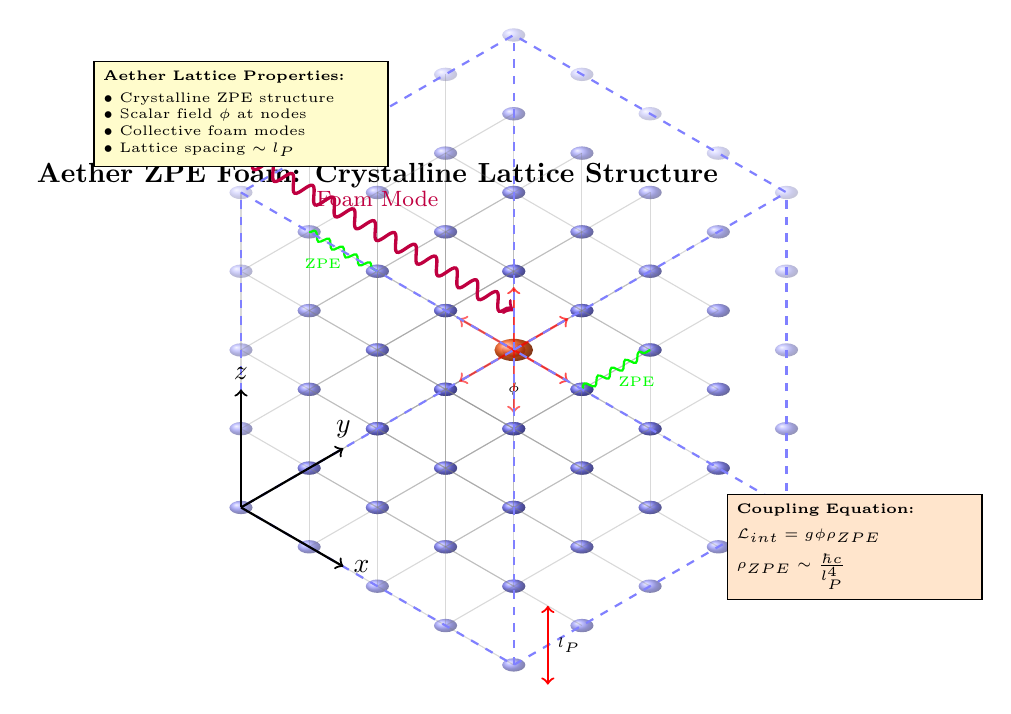
\begin{tikzpicture}[scale=1.0,
  x={(0.866cm,-0.5cm)}, y={(0.866cm,0.5cm)}, z={(0cm,1cm)}]

  % Title
  \node[anchor=north] at (2,0,5.5) {\textbf{Aether ZPE Foam: Crystalline Lattice Structure}};

  % 3D cubic lattice nodes (5x5x5 grid, showing subset)
  \foreach \x in {0,1,2,3,4} {
    \foreach \y in {0,1,2,3,4} {
      \foreach \z in {0,1,2,3,4} {
        % Draw spheres at lattice points
        \pgfmathsetmacro{\opacity}{0.6 - 0.08*\z}
        \shade[ball color=blue!60!white, opacity=\opacity] (\x,\y,\z) circle (0.12);
      }
    }
  }

  % Draw connecting edges (subset to avoid clutter)
  \foreach \x in {0,1,2,3} {
    \foreach \y in {0,1,2,3} {
      \foreach \z in {0,1,2,3} {
        \draw[gray, thin, opacity=0.3] (\x,\y,\z) -- (\x+1,\y,\z);
        \draw[gray, thin, opacity=0.3] (\x,\y,\z) -- (\x,\y+1,\z);
        \draw[gray, thin, opacity=0.3] (\x,\y,\z) -- (\x,\y,\z+1);
      }
    }
  }

  % Highlight central node with scalar field
  \shade[ball color=red!70!yellow, opacity=0.9] (2,2,2) circle (0.2);
  \node[font=\tiny, below] at (2,2,1.7) {$\phi$};

  % Scalar field coupling waves (emanating from center)
  \draw[red, thick, ->, opacity=0.7] (2,2,2) -- (2.8,2,2);
  \draw[red, thick, ->, opacity=0.7] (2,2,2) -- (2,2.8,2);
  \draw[red, thick, ->, opacity=0.7] (2,2,2) -- (2,2,2.8);
  \draw[red, thick, ->, opacity=0.6] (2,2,2) -- (1.2,2,2);
  \draw[red, thick, ->, opacity=0.6] (2,2,2) -- (2,1.2,2);
  \draw[red, thick, ->, opacity=0.6] (2,2,2) -- (2,2,1.2);

  % ZPE fluctuation annotation
  \draw[green, thick, decorate, decoration={snake, amplitude=0.5mm, segment length=2mm}]
    (0.5,0.5,3.5) -- (1.5,0.5,3.5);
  \node[font=\tiny, text=green] at (1,0.2,3.5) {ZPE};

  \draw[green, thick, decorate, decoration={snake, amplitude=0.5mm, segment length=2mm}]
    (3.5,1.5,2.5) -- (3.5,2.5,2.5);
  \node[font=\tiny, text=green] at (3.8,2,2.5) {ZPE};

  % Foam vibration mode (collective oscillation)
  \draw[purple, very thick, ->, decorate, decoration={snake, amplitude=1mm, segment length=3mm}]
    (0,0,4.5) -- (4,0,4.5);
  \node[font=\footnotesize, text=purple, above] at (2,0,4.7) {Foam Mode};

  % Crystalline structure box
  \draw[thick, dashed, blue!50] (0,0,0) -- (4,0,0) -- (4,4,0) -- (0,4,0) -- cycle;
  \draw[thick, dashed, blue!50] (0,0,4) -- (4,0,4) -- (4,4,4) -- (0,4,4) -- cycle;
  \draw[thick, dashed, blue!50] (0,0,0) -- (0,0,4);
  \draw[thick, dashed, blue!50] (4,0,0) -- (4,0,4);
  \draw[thick, dashed, blue!50] (4,4,0) -- (4,4,4);
  \draw[thick, dashed, blue!50] (0,4,0) -- (0,4,4);

  % Annotations outside the lattice
  \node[draw, rectangle, fill=yellow!20, font=\tiny, align=left, text width=3.5cm] at (-2,2,3) {
    \textbf{Aether Lattice Properties:} \\[2pt]
    $\bullet$ Crystalline ZPE structure \\
    $\bullet$ Scalar field $\phi$ at nodes \\
    $\bullet$ Collective foam modes \\
    $\bullet$ Lattice spacing $\sim l_P$
  };

  \node[draw, rectangle, fill=orange!20, font=\tiny, align=left, text width=3cm] at (7,2,2) {
    \textbf{Coupling Equation:} \\[3pt]
    $\mathcal{L}_{\text{int}} = g \phi \rho_{\text{ZPE}}$ \\[3pt]
    $\rho_{\text{ZPE}} \sim \frac{\hbar c}{l_P^4}$
  };

  % Axes labels
  \draw[->, thick] (0,0,0) -- (1.5,0,0) node[right] {$x$};
  \draw[->, thick] (0,0,0) -- (0,1.5,0) node[above] {$y$};
  \draw[->, thick] (0,0,0) -- (0,0,1.5) node[above] {$z$};

  % Scale indicator
  \draw[<->, thick, red] (4.5,0,0) -- (4.5,0,1);
  \node[right, font=\tiny] at (4.5,0,0.5) {$l_P$};

\end{tikzpicture}

% Usage: %==============================================================================
% Figure: Aether ZPE Foam 3D Visualization
% Source: Ch07-08 (Aether Framework)
% Framework: A (Aether) | Type: 3D lattice diagram
% Date: 2025-10-21
%==============================================================================

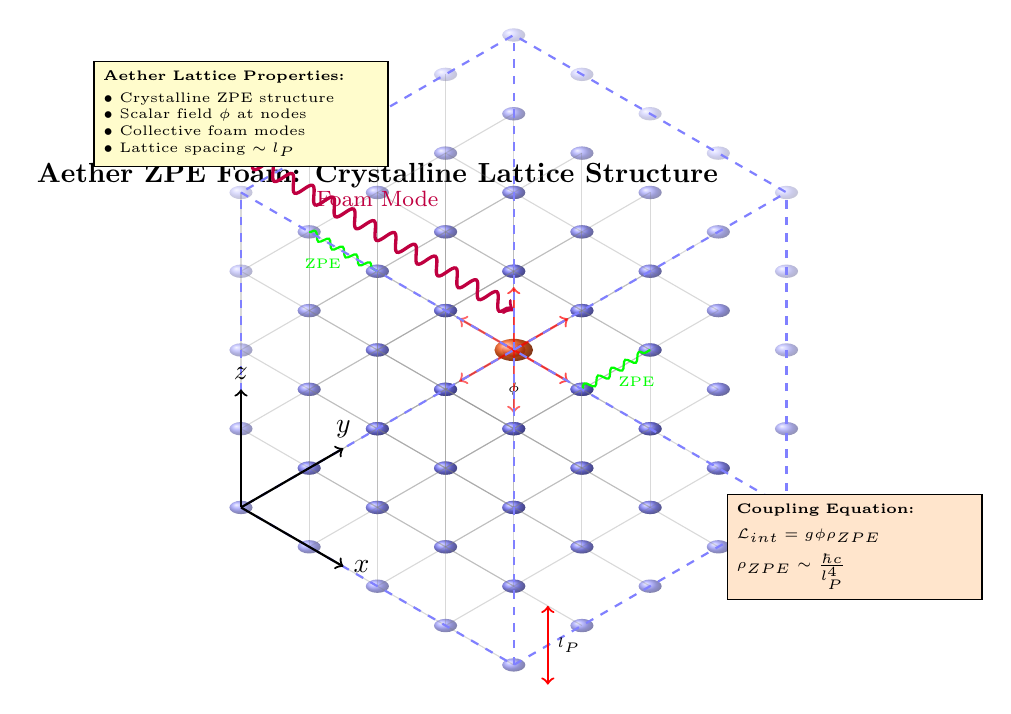
\begin{tikzpicture}[scale=1.0,
  x={(0.866cm,-0.5cm)}, y={(0.866cm,0.5cm)}, z={(0cm,1cm)}]

  % Title
  \node[anchor=north] at (2,0,5.5) {\textbf{Aether ZPE Foam: Crystalline Lattice Structure}};

  % 3D cubic lattice nodes (5x5x5 grid, showing subset)
  \foreach \x in {0,1,2,3,4} {
    \foreach \y in {0,1,2,3,4} {
      \foreach \z in {0,1,2,3,4} {
        % Draw spheres at lattice points
        \pgfmathsetmacro{\opacity}{0.6 - 0.08*\z}
        \shade[ball color=blue!60!white, opacity=\opacity] (\x,\y,\z) circle (0.12);
      }
    }
  }

  % Draw connecting edges (subset to avoid clutter)
  \foreach \x in {0,1,2,3} {
    \foreach \y in {0,1,2,3} {
      \foreach \z in {0,1,2,3} {
        \draw[gray, thin, opacity=0.3] (\x,\y,\z) -- (\x+1,\y,\z);
        \draw[gray, thin, opacity=0.3] (\x,\y,\z) -- (\x,\y+1,\z);
        \draw[gray, thin, opacity=0.3] (\x,\y,\z) -- (\x,\y,\z+1);
      }
    }
  }

  % Highlight central node with scalar field
  \shade[ball color=red!70!yellow, opacity=0.9] (2,2,2) circle (0.2);
  \node[font=\tiny, below] at (2,2,1.7) {$\phi$};

  % Scalar field coupling waves (emanating from center)
  \draw[red, thick, ->, opacity=0.7] (2,2,2) -- (2.8,2,2);
  \draw[red, thick, ->, opacity=0.7] (2,2,2) -- (2,2.8,2);
  \draw[red, thick, ->, opacity=0.7] (2,2,2) -- (2,2,2.8);
  \draw[red, thick, ->, opacity=0.6] (2,2,2) -- (1.2,2,2);
  \draw[red, thick, ->, opacity=0.6] (2,2,2) -- (2,1.2,2);
  \draw[red, thick, ->, opacity=0.6] (2,2,2) -- (2,2,1.2);

  % ZPE fluctuation annotation
  \draw[green, thick, decorate, decoration={snake, amplitude=0.5mm, segment length=2mm}]
    (0.5,0.5,3.5) -- (1.5,0.5,3.5);
  \node[font=\tiny, text=green] at (1,0.2,3.5) {ZPE};

  \draw[green, thick, decorate, decoration={snake, amplitude=0.5mm, segment length=2mm}]
    (3.5,1.5,2.5) -- (3.5,2.5,2.5);
  \node[font=\tiny, text=green] at (3.8,2,2.5) {ZPE};

  % Foam vibration mode (collective oscillation)
  \draw[purple, very thick, ->, decorate, decoration={snake, amplitude=1mm, segment length=3mm}]
    (0,0,4.5) -- (4,0,4.5);
  \node[font=\footnotesize, text=purple, above] at (2,0,4.7) {Foam Mode};

  % Crystalline structure box
  \draw[thick, dashed, blue!50] (0,0,0) -- (4,0,0) -- (4,4,0) -- (0,4,0) -- cycle;
  \draw[thick, dashed, blue!50] (0,0,4) -- (4,0,4) -- (4,4,4) -- (0,4,4) -- cycle;
  \draw[thick, dashed, blue!50] (0,0,0) -- (0,0,4);
  \draw[thick, dashed, blue!50] (4,0,0) -- (4,0,4);
  \draw[thick, dashed, blue!50] (4,4,0) -- (4,4,4);
  \draw[thick, dashed, blue!50] (0,4,0) -- (0,4,4);

  % Annotations outside the lattice
  \node[draw, rectangle, fill=yellow!20, font=\tiny, align=left, text width=3.5cm] at (-2,2,3) {
    \textbf{Aether Lattice Properties:} \\[2pt]
    $\bullet$ Crystalline ZPE structure \\
    $\bullet$ Scalar field $\phi$ at nodes \\
    $\bullet$ Collective foam modes \\
    $\bullet$ Lattice spacing $\sim l_P$
  };

  \node[draw, rectangle, fill=orange!20, font=\tiny, align=left, text width=3cm] at (7,2,2) {
    \textbf{Coupling Equation:} \\[3pt]
    $\mathcal{L}_{\text{int}} = g \phi \rho_{\text{ZPE}}$ \\[3pt]
    $\rho_{\text{ZPE}} \sim \frac{\hbar c}{l_P^4}$
  };

  % Axes labels
  \draw[->, thick] (0,0,0) -- (1.5,0,0) node[right] {$x$};
  \draw[->, thick] (0,0,0) -- (0,1.5,0) node[above] {$y$};
  \draw[->, thick] (0,0,0) -- (0,0,1.5) node[above] {$z$};

  % Scale indicator
  \draw[<->, thick, red] (4.5,0,0) -- (4.5,0,1);
  \node[right, font=\tiny] at (4.5,0,0.5) {$l_P$};

\end{tikzpicture}

% Usage: %==============================================================================
% Figure: Aether ZPE Foam 3D Visualization
% Source: Ch07-08 (Aether Framework)
% Framework: A (Aether) | Type: 3D lattice diagram
% Date: 2025-10-21
%==============================================================================

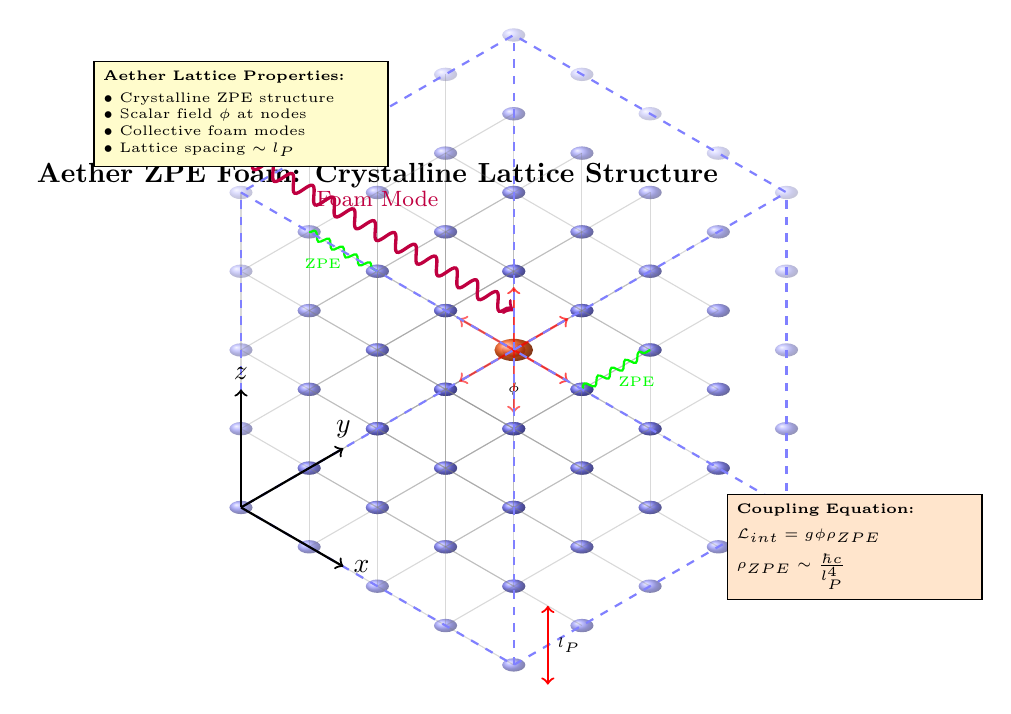
\begin{tikzpicture}[scale=1.0,
  x={(0.866cm,-0.5cm)}, y={(0.866cm,0.5cm)}, z={(0cm,1cm)}]

  % Title
  \node[anchor=north] at (2,0,5.5) {\textbf{Aether ZPE Foam: Crystalline Lattice Structure}};

  % 3D cubic lattice nodes (5x5x5 grid, showing subset)
  \foreach \x in {0,1,2,3,4} {
    \foreach \y in {0,1,2,3,4} {
      \foreach \z in {0,1,2,3,4} {
        % Draw spheres at lattice points
        \pgfmathsetmacro{\opacity}{0.6 - 0.08*\z}
        \shade[ball color=blue!60!white, opacity=\opacity] (\x,\y,\z) circle (0.12);
      }
    }
  }

  % Draw connecting edges (subset to avoid clutter)
  \foreach \x in {0,1,2,3} {
    \foreach \y in {0,1,2,3} {
      \foreach \z in {0,1,2,3} {
        \draw[gray, thin, opacity=0.3] (\x,\y,\z) -- (\x+1,\y,\z);
        \draw[gray, thin, opacity=0.3] (\x,\y,\z) -- (\x,\y+1,\z);
        \draw[gray, thin, opacity=0.3] (\x,\y,\z) -- (\x,\y,\z+1);
      }
    }
  }

  % Highlight central node with scalar field
  \shade[ball color=red!70!yellow, opacity=0.9] (2,2,2) circle (0.2);
  \node[font=\tiny, below] at (2,2,1.7) {$\phi$};

  % Scalar field coupling waves (emanating from center)
  \draw[red, thick, ->, opacity=0.7] (2,2,2) -- (2.8,2,2);
  \draw[red, thick, ->, opacity=0.7] (2,2,2) -- (2,2.8,2);
  \draw[red, thick, ->, opacity=0.7] (2,2,2) -- (2,2,2.8);
  \draw[red, thick, ->, opacity=0.6] (2,2,2) -- (1.2,2,2);
  \draw[red, thick, ->, opacity=0.6] (2,2,2) -- (2,1.2,2);
  \draw[red, thick, ->, opacity=0.6] (2,2,2) -- (2,2,1.2);

  % ZPE fluctuation annotation
  \draw[green, thick, decorate, decoration={snake, amplitude=0.5mm, segment length=2mm}]
    (0.5,0.5,3.5) -- (1.5,0.5,3.5);
  \node[font=\tiny, text=green] at (1,0.2,3.5) {ZPE};

  \draw[green, thick, decorate, decoration={snake, amplitude=0.5mm, segment length=2mm}]
    (3.5,1.5,2.5) -- (3.5,2.5,2.5);
  \node[font=\tiny, text=green] at (3.8,2,2.5) {ZPE};

  % Foam vibration mode (collective oscillation)
  \draw[purple, very thick, ->, decorate, decoration={snake, amplitude=1mm, segment length=3mm}]
    (0,0,4.5) -- (4,0,4.5);
  \node[font=\footnotesize, text=purple, above] at (2,0,4.7) {Foam Mode};

  % Crystalline structure box
  \draw[thick, dashed, blue!50] (0,0,0) -- (4,0,0) -- (4,4,0) -- (0,4,0) -- cycle;
  \draw[thick, dashed, blue!50] (0,0,4) -- (4,0,4) -- (4,4,4) -- (0,4,4) -- cycle;
  \draw[thick, dashed, blue!50] (0,0,0) -- (0,0,4);
  \draw[thick, dashed, blue!50] (4,0,0) -- (4,0,4);
  \draw[thick, dashed, blue!50] (4,4,0) -- (4,4,4);
  \draw[thick, dashed, blue!50] (0,4,0) -- (0,4,4);

  % Annotations outside the lattice
  \node[draw, rectangle, fill=yellow!20, font=\tiny, align=left, text width=3.5cm] at (-2,2,3) {
    \textbf{Aether Lattice Properties:} \\[2pt]
    $\bullet$ Crystalline ZPE structure \\
    $\bullet$ Scalar field $\phi$ at nodes \\
    $\bullet$ Collective foam modes \\
    $\bullet$ Lattice spacing $\sim l_P$
  };

  \node[draw, rectangle, fill=orange!20, font=\tiny, align=left, text width=3cm] at (7,2,2) {
    \textbf{Coupling Equation:} \\[3pt]
    $\mathcal{L}_{\text{int}} = g \phi \rho_{\text{ZPE}}$ \\[3pt]
    $\rho_{\text{ZPE}} \sim \frac{\hbar c}{l_P^4}$
  };

  % Axes labels
  \draw[->, thick] (0,0,0) -- (1.5,0,0) node[right] {$x$};
  \draw[->, thick] (0,0,0) -- (0,1.5,0) node[above] {$y$};
  \draw[->, thick] (0,0,0) -- (0,0,1.5) node[above] {$z$};

  % Scale indicator
  \draw[<->, thick, red] (4.5,0,0) -- (4.5,0,1);
  \node[right, font=\tiny] at (4.5,0,0.5) {$l_P$};

\end{tikzpicture}

% Usage: %==============================================================================
% Figure: Aether ZPE Foam 3D Visualization
% Source: Ch07-08 (Aether Framework)
% Framework: A (Aether) | Type: 3D lattice diagram
% Date: 2025-10-21
%==============================================================================

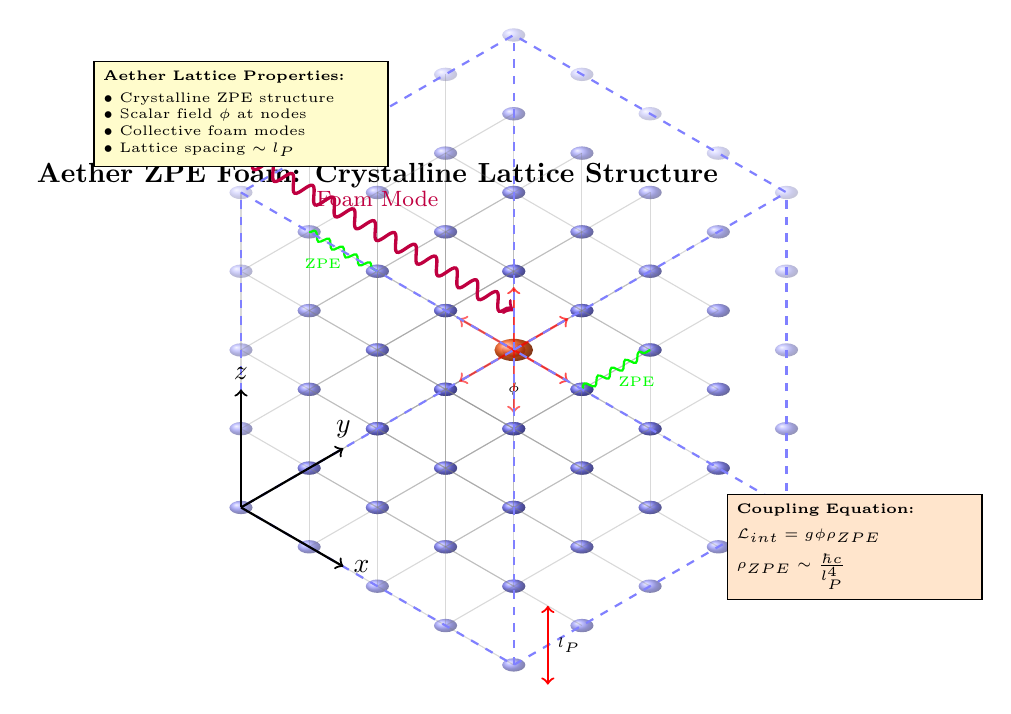
\begin{tikzpicture}[scale=1.0,
  x={(0.866cm,-0.5cm)}, y={(0.866cm,0.5cm)}, z={(0cm,1cm)}]

  % Title
  \node[anchor=north] at (2,0,5.5) {\textbf{Aether ZPE Foam: Crystalline Lattice Structure}};

  % 3D cubic lattice nodes (5x5x5 grid, showing subset)
  \foreach \x in {0,1,2,3,4} {
    \foreach \y in {0,1,2,3,4} {
      \foreach \z in {0,1,2,3,4} {
        % Draw spheres at lattice points
        \pgfmathsetmacro{\opacity}{0.6 - 0.08*\z}
        \shade[ball color=blue!60!white, opacity=\opacity] (\x,\y,\z) circle (0.12);
      }
    }
  }

  % Draw connecting edges (subset to avoid clutter)
  \foreach \x in {0,1,2,3} {
    \foreach \y in {0,1,2,3} {
      \foreach \z in {0,1,2,3} {
        \draw[gray, thin, opacity=0.3] (\x,\y,\z) -- (\x+1,\y,\z);
        \draw[gray, thin, opacity=0.3] (\x,\y,\z) -- (\x,\y+1,\z);
        \draw[gray, thin, opacity=0.3] (\x,\y,\z) -- (\x,\y,\z+1);
      }
    }
  }

  % Highlight central node with scalar field
  \shade[ball color=red!70!yellow, opacity=0.9] (2,2,2) circle (0.2);
  \node[font=\tiny, below] at (2,2,1.7) {$\phi$};

  % Scalar field coupling waves (emanating from center)
  \draw[red, thick, ->, opacity=0.7] (2,2,2) -- (2.8,2,2);
  \draw[red, thick, ->, opacity=0.7] (2,2,2) -- (2,2.8,2);
  \draw[red, thick, ->, opacity=0.7] (2,2,2) -- (2,2,2.8);
  \draw[red, thick, ->, opacity=0.6] (2,2,2) -- (1.2,2,2);
  \draw[red, thick, ->, opacity=0.6] (2,2,2) -- (2,1.2,2);
  \draw[red, thick, ->, opacity=0.6] (2,2,2) -- (2,2,1.2);

  % ZPE fluctuation annotation
  \draw[green, thick, decorate, decoration={snake, amplitude=0.5mm, segment length=2mm}]
    (0.5,0.5,3.5) -- (1.5,0.5,3.5);
  \node[font=\tiny, text=green] at (1,0.2,3.5) {ZPE};

  \draw[green, thick, decorate, decoration={snake, amplitude=0.5mm, segment length=2mm}]
    (3.5,1.5,2.5) -- (3.5,2.5,2.5);
  \node[font=\tiny, text=green] at (3.8,2,2.5) {ZPE};

  % Foam vibration mode (collective oscillation)
  \draw[purple, very thick, ->, decorate, decoration={snake, amplitude=1mm, segment length=3mm}]
    (0,0,4.5) -- (4,0,4.5);
  \node[font=\footnotesize, text=purple, above] at (2,0,4.7) {Foam Mode};

  % Crystalline structure box
  \draw[thick, dashed, blue!50] (0,0,0) -- (4,0,0) -- (4,4,0) -- (0,4,0) -- cycle;
  \draw[thick, dashed, blue!50] (0,0,4) -- (4,0,4) -- (4,4,4) -- (0,4,4) -- cycle;
  \draw[thick, dashed, blue!50] (0,0,0) -- (0,0,4);
  \draw[thick, dashed, blue!50] (4,0,0) -- (4,0,4);
  \draw[thick, dashed, blue!50] (4,4,0) -- (4,4,4);
  \draw[thick, dashed, blue!50] (0,4,0) -- (0,4,4);

  % Annotations outside the lattice
  \node[draw, rectangle, fill=yellow!20, font=\tiny, align=left, text width=3.5cm] at (-2,2,3) {
    \textbf{Aether Lattice Properties:} \\[2pt]
    $\bullet$ Crystalline ZPE structure \\
    $\bullet$ Scalar field $\phi$ at nodes \\
    $\bullet$ Collective foam modes \\
    $\bullet$ Lattice spacing $\sim l_P$
  };

  \node[draw, rectangle, fill=orange!20, font=\tiny, align=left, text width=3cm] at (7,2,2) {
    \textbf{Coupling Equation:} \\[3pt]
    $\mathcal{L}_{\text{int}} = g \phi \rho_{\text{ZPE}}$ \\[3pt]
    $\rho_{\text{ZPE}} \sim \frac{\hbar c}{l_P^4}$
  };

  % Axes labels
  \draw[->, thick] (0,0,0) -- (1.5,0,0) node[right] {$x$};
  \draw[->, thick] (0,0,0) -- (0,1.5,0) node[above] {$y$};
  \draw[->, thick] (0,0,0) -- (0,0,1.5) node[above] {$z$};

  % Scale indicator
  \draw[<->, thick, red] (4.5,0,0) -- (4.5,0,1);
  \node[right, font=\tiny] at (4.5,0,0.5) {$l_P$};

\end{tikzpicture}

% Usage: \input{modules/figures/fig_aether_zpe_foam_3d.tex}
% Notes: 3D visualization of Aether framework's crystalline ZPE foam structure
%        showing lattice nodes, scalar field coupling, and collective vibration modes.
%==============================================================================

% Notes: 3D visualization of Aether framework's crystalline ZPE foam structure
%        showing lattice nodes, scalar field coupling, and collective vibration modes.
%==============================================================================

% Notes: 3D visualization of Aether framework's crystalline ZPE foam structure
%        showing lattice nodes, scalar field coupling, and collective vibration modes.
%==============================================================================

% Notes: 3D visualization of Aether framework's crystalline ZPE foam structure
%        showing lattice nodes, scalar field coupling, and collective vibration modes.
%==============================================================================
